\documentclass[a4paper,11pt,twoside,openright]{report}

\usepackage{graphicx}
%\usepackage{ngerman}
\usepackage[utf8x]{inputenc}
\usepackage{fancyvrb}
\usepackage{courier}
\usepackage{helvet}
\usepackage{tikz}
\usepackage{xcolor}
\usepackage{pdfpages}
\usepackage[strict]{changepage}
\usepackage{xspace}
\usepackage{hyperref}
\usepackage{cleveref}
\usetikzlibrary{shapes.geometric}
\usetikzlibrary{arrows}
\usepackage{subcaption} 

\pdfoptionpdfminorversion=6

% \definecolor{se_dark_blue}{RGB}{0,103,166} % powerpoint
\definecolor{se_dark_blue}{RGB}{0,96,178} % website
% \definecolor{se_light_blue}{RGB}{119,158,201} % powerpoint
\definecolor{se_light_blue}{RGB}{129,160,225} % website


%% setup listings
\usepackage{listings}
\lstset{
    numbers=left,
    numberstyle=\tiny,
    numbersep=5pt,
    xleftmargin=11pt,
    xrightmargin=4pt,
    frame=single,
    aboveskip=0pt,
    belowskip=-6pt,
    sensitive=true,
    float=!t,
    breaklines=false,
    captionpos=b,
    tabsize=2,
    showstringspaces=false,
    basicstyle=\small\ttfamily,
    morecomment=[l]{//},
    morecomment=[s][\itshape]{/**}{*/}
}

%% defines the listings laguage named 'MontiArc' derived from the language 'Java' 
%% adding the below listed keywords. See 
%% ftp://ftp.tex.ac.uk/tex-archive/macros/latex/contrib/listings/listings.pdf
%% for listings documentation
\lstdefinelanguage{MontiArc}[]{Java}{
  morekeywords={component, port, in, out, inv, package, import, connect, autoconnect}
}

% Seite einrichten
\setlength{\voffset}{-1in}
\setlength{\hoffset}{-1in}

\setlength{\topmargin}{2.5cm}		   
\setlength{\headheight}{0cm}		   
\setlength{\headsep}{0cm}		   
\setlength{\oddsidemargin}{3,3cm}  % innen ein wenig mehr Rand für die Klebebindung
\setlength{\evensidemargin}{2,7cm} % dafür außen ein wenig weniger
\setlength{\textwidth}{15cm}		   
\setlength{\textheight}{23,5cm}		   
\setlength{\parindent}{0cm}

% own commands
\newcommand{\red}[1]{\color{red}#1\color{black}}
\newcommand{\todoLine}{\noindent\rule{15cm}{0.4pt}}
\newcommand{\todo}[1]{\todoLine\\\red{TODO:}#1 \todoLine}

% Words
\newcommand{\emptyLine}{{\LARGE ~\\}}
\newcommand{\MontiCar}{MontiCar\xspace}
\newcommand{\kitti}{KITTI\xspace}
\newcommand{\cnnarch}{CNNArch\xspace}
\newcommand{\alexnet}{AlexNet\xspace}
\newcommand{\nn}{neural network\xspace}
\newcommand{\nns}{neural networks\xspace}
\newcommand{\alvinn}{ALVINN\xspace}


\begin{document}

% Einrücken von Absätzen verhindern und 1.5 Zeilen Absatzabstand
\setlength{\parindent}{0pt}
\setlength{\parskip}{1.5ex plus0.5ex minus0.5ex}

%% Dieses Teildokument beschreibt die Titelseite.
%

% Seitenzähler auf 1, Römische Ziffern.
\setcounter{page}{1}
\pagenumbering{roman}

\thispagestyle{headings}

%\changepage{<text height>}{<text width>}{<even-side margin>}{<odd-side margin>}{<column sep.>}{<topmargin>}{<headheight>}{<headsep>}{<footskip>}
\changepage{5,1cm}{2.4cm}{}{-0.7cm}{}{-2,3cm}{}{}{}

% Eigentliche Titelseite.
\begin{titlepage}
	
\begin{figure}\raggedleft
\includegraphics[height=3.0cm]{src/pic/logo.jpg}\end{figure}
  
\begin{tikzpicture}[overlay]

% horizontal lines
\draw[color=se_dark_blue, thick] (-1.6, 0.9) -- (17.4, 0.9);
\draw[color=se_light_blue, thick] (-1.4, 0.7) -- (17.4, 0.7);

% vertical lines
\draw[color=se_dark_blue, thick] (-1, 0.9) -- (-1, -24.5);
\draw[color=se_light_blue, thick] (-0.8, 0.7) -- (-0.8, -24.5);

\end{tikzpicture}

\vspace*{-1.5em}

\begin{flushleft}
  {\fontfamily{phv}  
  	{\LARGE
      Rheinisch Westfälische Technische Hochschule Aachen \\
      Lehrstuhl für Software Engineering \\}
    \vspace{3em}
  
    {\LARGE \textbf{Erste Titel-Zeile}\\} 
    {\LARGE \textbf{Zweite Titel-Zeile}\\} 
    {\LARGE \textbf{Dritte Titel-Zeile}\\} % Oder \emptyLine falls nicht Titel kürzer
    {\LARGE \textbf{Vierte Titel-Zeile}\\} % Oder \emptyLine falls nicht Titel kürzer
    \vspace{3em}
		
    {\Large \textbf{Diplomarbeit/Masterarbeit/Studienarbeit}\\}
		\vspace{3em} 
		
		{\large von\\} % presented by
    
    {\LARGE \textbf{Name, Vorname}\\}
    \vspace{3em} 
		    
    {\Large \textbf{1. Prüfer: Prof.\ Dr.\ B.\ Rumpe}\\}
    \vspace{1em} 
    {\Large \textbf{2. Prüfer: }\\}
    \vspace{1em} 
    {\Large \textbf{Betreuer: }\\}
    \vspace{7em} 

    {\large Diese Arbeit wurde vorgelegt am Lehrstuhl für Software Engineering \\}
    \vspace{1em}
    % The present work was submitted to the chair of software engineering
		{\large	Aachen, den \today\\}
  }
\end{flushleft}

\end{titlepage}

\changepage{-5,1cm}{-2.4cm}{}{0.7cm}{}{2,3cm}{}{}{}





 %Dieses Teildokument beschreibt die Titelseite.
%

% Seitenzähler auf 1, Römische Ziffern.
\setcounter{page}{1}
\pagenumbering{roman}

\thispagestyle{headings}

%\changepage{<text height>}{<text width>}{<even-side margin>}{<odd-side margin>}{<column sep.>}{<topmargin>}{<headheight>}{<headsep>}{<footskip>}
\changepage{5,1cm}{2.4cm}{}{-0.7cm}{}{-2,3cm}{}{}{}

% Eigentliche Titelseite.
\begin{titlepage}
	
\begin{figure}\raggedleft
\includegraphics[height=3.0cm]{src/pic/logo.jpg}\end{figure}
  
\begin{tikzpicture}[overlay]

% horizontal lines
\draw[color=se_dark_blue, thick] (-1.6, 0.9) -- (17.4, 0.9);
\draw[color=se_light_blue, thick] (-1.4, 0.7) -- (17.4, 0.7);

% vertical lines
\draw[color=se_dark_blue, thick] (-1, 0.9) -- (-1, -24.5);
\draw[color=se_light_blue, thick] (-0.8, 0.7) -- (-0.8, -24.5);

\end{tikzpicture}

\vspace*{-1.5em}

\begin{flushleft}
  {\fontfamily{phv}  
  	{\LARGE
      RWTH Aachen University \\
      Software Engineering Group \\}
    \vspace{3em}
  
    {\LARGE \textbf{Deep Learning in Autonomous Driving}\\} 
    {\LARGE \textbf{Direct Perception Approach}\\} 
    {\LARGE \textbf{ }\\} % Replace with \emptyLine if title is shorter
    {\LARGE \textbf{ }\\} % Replace with \emptyLine if title is shorter
    \vspace{3em}
		
    {\Large \textbf{Seminar Paper}\\}
		\vspace{3em} 
		
		{\large presented by\\} 
    
    {\LARGE \textbf{Bergerbusch, Timo}\\}
    \vspace{3em} 
		    
    {\Large \textbf{1st Examiner: Prof.\ Dr.\ B.\ Rumpe}\\}
    \vspace{1em} 
%    {\Large \textbf{2nd Examiner: }\\}
%    \vspace{1em} 
    {\Large \textbf{Advisor: Evgeny Kusmenko}\\}
    \vspace{7em} 

    {\large The present work was submitted to the Chair of Software Engineering \\}
    \vspace{1em}
    % The present work was submitted to the chair of software engineering
		{\large	Aachen, \today\\}
  }
\end{flushleft}

\end{titlepage}

\changepage{-5,1cm}{-2.4cm}{}{0.7cm}{}{2,3cm}{}{}{}




 % English cover

\clearpage

% Erklaerung

%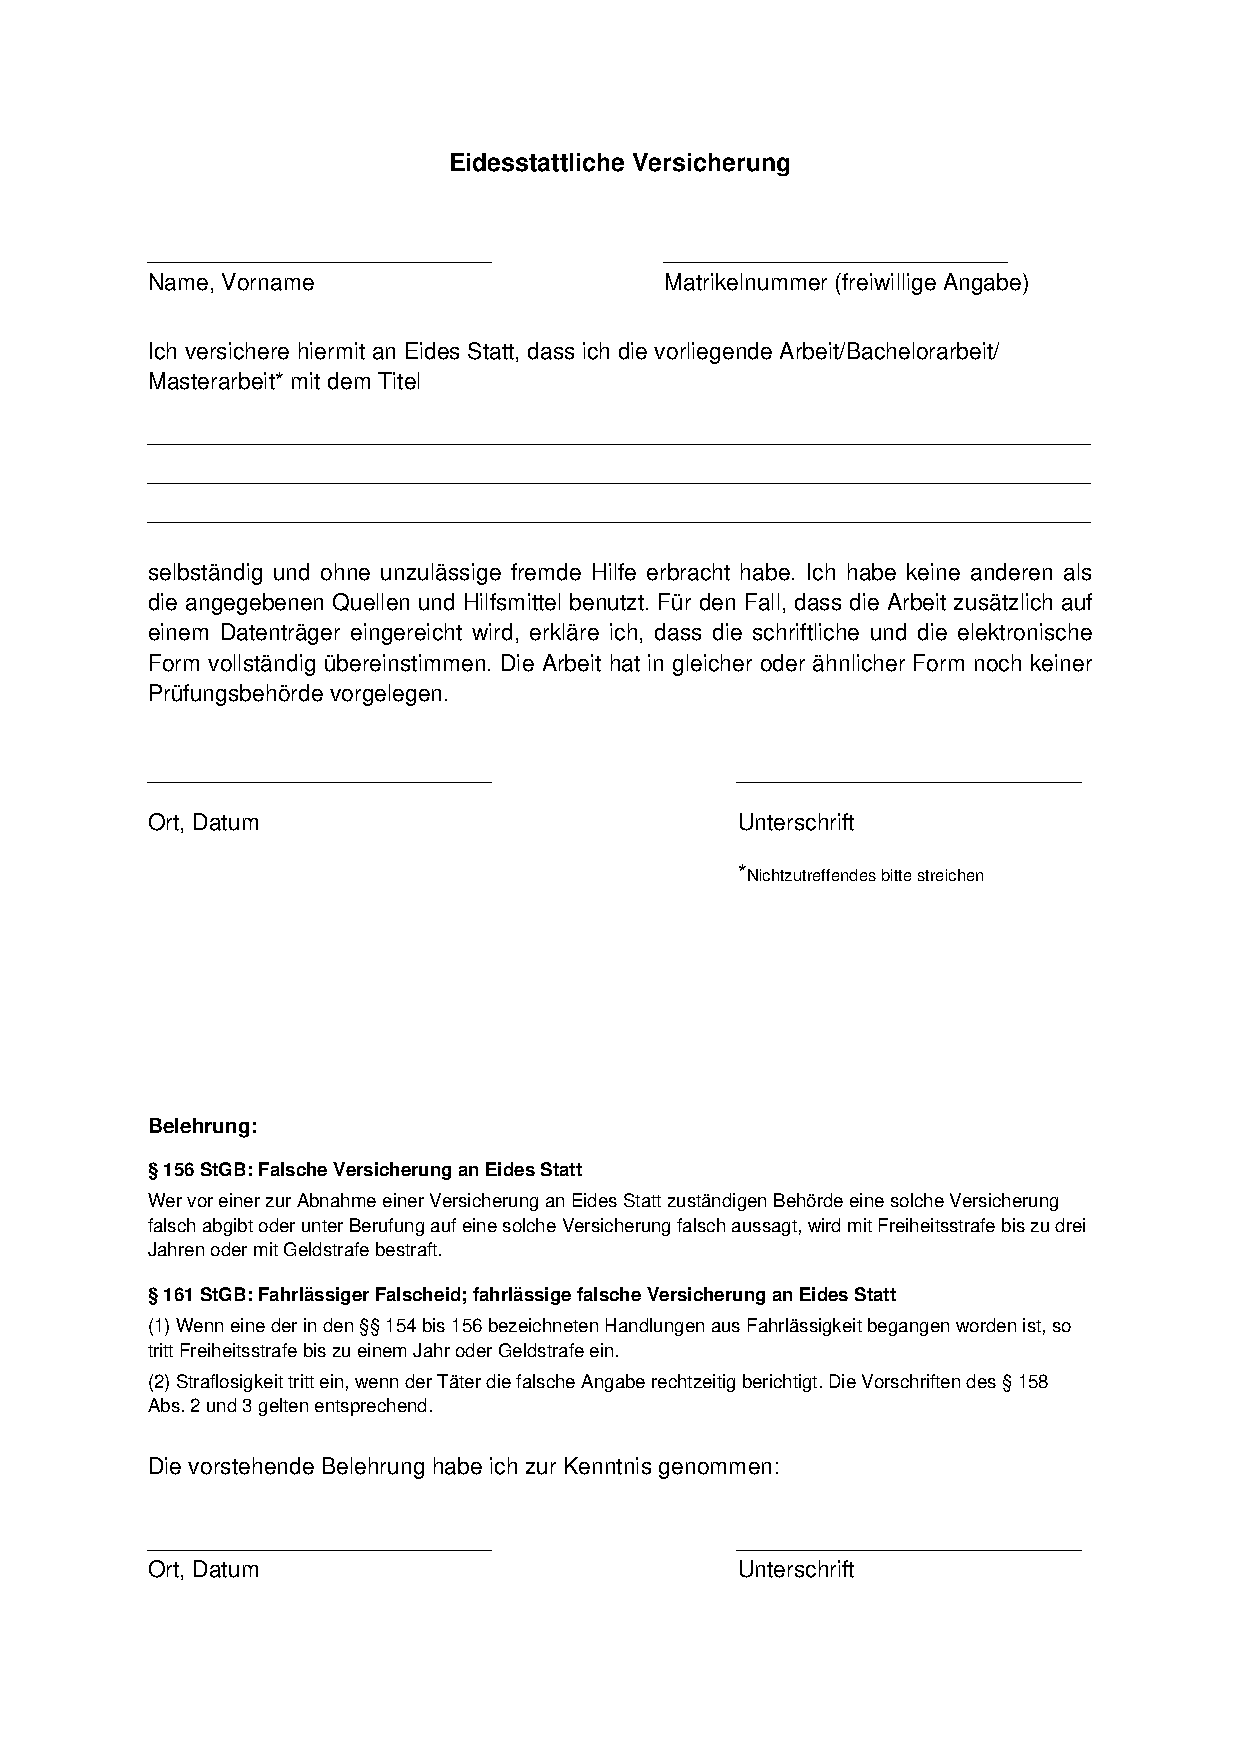
\includepdf[pages={1},offset=-1in -1in]{Formular_Eidesstattliche_Versicherung_neu.pdf}
 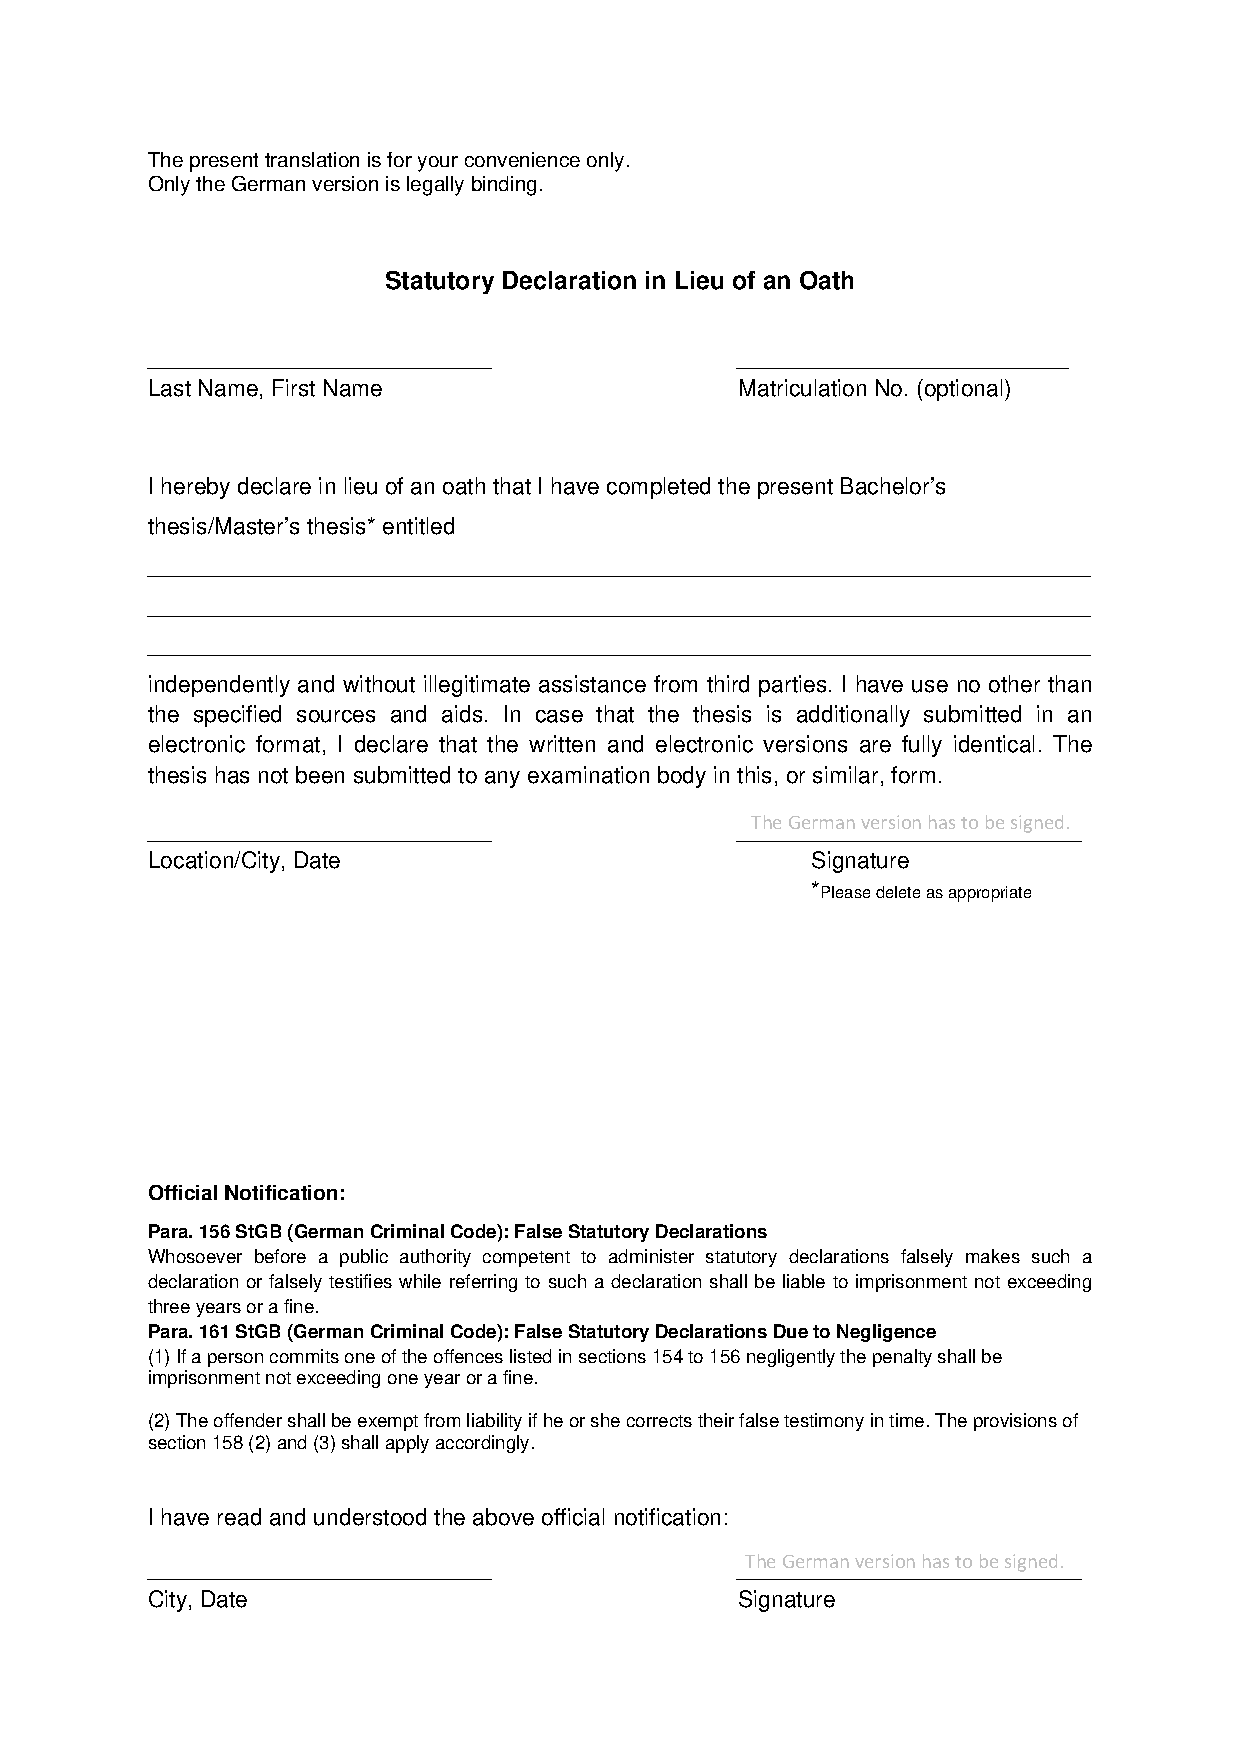
\includepdf[pages={1},offset=-1in -1in]{Statutory_Declaration_in_Lieu_of_an_Oath.pdf} % English 

\clearpage

%TODO rewrite
{\bf\Large Abstract} \\ [1em]
The topic of autonomous driving using artificial intelligence increases in importance with the overwhelming amount of software usage within vehicles. For that \textit{Convolutional Neural Networks} (CNNs), which try to figure out the importance of special areas of a single picture, have been shown to be promising. \\
In this paper we will give a general introduction to the topic of \nns and then state the specialties defining a CNN.
We distinguish between the three main paradigms currently used and researched for autonomous driving agents: mediated perception, behavior reflex and direct perception.\\
Further we will compare different domain specific languages \cnnarch, \caffe, \caffetwo and \mxnet, based on the factors of usability, scope of functionality, also regarding training possibilities, and the integration on a subject.

We will analyze a CNN using the direct perception approach, in different languages, and compare it to state-of-the-art implementations of the other paradigms, training on a simulator \torcs or the \kitti database. Furthermore we state scenarios probably causing problems for the direct perception approach. 

Finally we create an overview of the mentioned languages with a table, which states the functionalities and properties in a nutshell.
\cleardoublepage


%\vspace*{2cm}
{\bf\Large Aufgabenstellung}

\cleardoublepage


\tableofcontents

\clearpage

% Ab erstem Kapitel Seiten arabisch zählen
\setcounter{page}{1}
\pagenumbering{arabic}

\chapter{Introduction}



\chapter{Comparison: \cnnarch \& \caffe}\label{chapter: Comparison}

In this chapter we want to compare the \alexnet (c.f. \Cref{sec: AlexNet}) implemented using \cnnarch and \caffe. This net is used in the direct perception approach (c.f. \Cref{sec: Direct Perception}) and therefore crucial for its performance. For both we take an in depth look at the predefined architecture by their respective language. We do that, since both implementations are done by language experts and build to be as efficient and precise in the language as possible.

Further, we state the currently most used methods to train an autonomous driving agent. Those training methods are also used for the approaches in \Cref{chapter: Deep Learning Approaches}. The important properties required are stated.


\section{Implementation} \label{sec: Implementation}

\subsection{\caffe} \label{subsec: Caffe Implementation}
The implementation of the \alexnet using \caffe is given partly in \Cref{lst: Caffe AlexNet}. The whole net has a total number of 284 lines. Obviously the code was written very verbosely. Every layer has to be explicitly specified, even if they have a very similar structure to a previous layer.

%\newpage  %TODO restructure
For example comparing the pooling layer ``pool1'' from line 51 to 61 and the pooling layer ``pool2'' from line 99 to 109 in \Cref{lst: pool1 and pool2}:
\begin{figure}[H]
	\centering
	\begin{subfigure}[b]{0.45\textwidth}
		\hspace*{2cm}\vdots
		\lstinputlisting[numbers=left, firstnumber = 51, basicstyle=\scriptsize,firstline=51, lastline=61]{src/listing/alexnet.prototxt}
		\hspace*{2cm}\vdots
		\caption{``pool1''}
		\label{lst: pool1}
	\end{subfigure}
	\begin{subfigure}[b]{0.45\textwidth}
		\hspace*{2cm}\vdots
		\lstinputlisting[numbers=left, firstnumber = 99, basicstyle=\scriptsize,firstline=99, lastline=109]{src/listing/alexnet.prototxt}
		\hspace*{2cm}\vdots
		\caption{``pool2''}
		\label{lst: pool2}
	\end{subfigure}
	\caption{}
	\label{lst: pool1 and pool2}
\end{figure}
The lines first 3 and last 6 lines are completely similar. The other 2 lines are just different regarding the name of the incoming and outgoing connections. Creating a huge and deep net would lead to an enormously large description file. 

\subsection{\cnnarch} \label{subsec: CNNArch Implementation}

The implementation of the \alexnet using \cnnarch can be seen in \Cref{lst: CNNArchLang AlexNet}. The complete script has 43 lines and defines the same net construction as the 284 line definition in \caffe. This shows the efficient language design used in the creation of \cnnarch (c.f. \Cref{sec: CNNArch}). \\
The two pooling operations of \Cref{lst: pool1 and pool2} can be located in line 32 using the Python like syntax of definition and the sequential connection \texttt{->} (c.f. \Cref{item: sequential connection}).

Using those techniques \cnnarch is able to write even complex \nn using a few lines of code. This and the syntax itself create an easy to read program.

\subsection{Comparison}
Due to complications regarding the \cnnarch-inclusion in an existing program infrastructure, as well as \caffe, currently having issues with their build-script there is no possibility to directly compare times taken for training the \nn. \\
Nevertheless based on the usage of \mxnet, by \cnnarch (c.f. \Cref{subsec: CNNArch Implementation} and \Cref{chapter: conclusion}), it is suspected to be much faster than the \caffe approach.\\
About the effectiveness and other performance indicators, such as error rate, there can not be any profound reasoning without an actual implementation and testing.

\section{Training}

In order to train a CNN, independent of the underlying approach (c.f. \Cref{chapter: DLL}), one has to obtain a huge database of input images and the labels, i.e. actions or values the CNN should have computed. For autonomous driving the training has to be rigorous. Otherwise the car driven by the agent will take damage by just slight changes of the circumstances.\\
Also different scenarios have to be trained. Only training the driving on a road without other cars and simply following the lane is a very disparate task compared to overtaking a slower car.\\
For that, the following sources of such databases are currently state-of-the-art.

\subsection{KITTI Dataset} \label{subsec: KITTI}

The \kitti dataset is a 6 hour recoding by the Karlsruhe Institute of Technology. They mounted various cameras and laser scanners on a VW Passat and drove around the german city Karlsruhe.\\
During those hours they collected a total amount of 180 GB of data. This data includes images, in different channels from the drivers point of view, sensor data of distances, steering angle, acceleration/braking, current speed, GPS coordinates, and others. \\
While other test sets are often developed using a very specific setup for a corresponding approach, the \kitti dataset has such a high variety of data captured, resulting in many appearances in other scientific papers. It has become one of the default datasets to compare different approaches on. \cite{KITTI}

\subsection{TORCS} \label{subsec: TORCS}

A game called \textbf{T}he \textbf{O}pen \textbf{R}acing \textbf{C}ar \textbf{S}imulator or short \torcs is a racing game specially designed for artificial intelligence research. It is designed to be modular in order to retrieve every kind of data one needs for their approach. It also offers a documented API, to create for example a driving agent. 

The possibility to collect any kind of data is what makes this game so popular in current research. The advantage over the \kitti dataset is that, if one needs a very specific value not included within the \kitti dataset, the approach can not be trained with it. Neglecting, whether such a value is meaningful in terms of the ability to collect it during real driving, there would be an other specialized set collecting only the data this specific approach needs. But this specialized set may lack a value, which is required in order to compare it with an another approach. So there is no common training set, on which a comparison could base.

% and maybe not collecting the data one needs to compare it to an other approach.

The disadvantage of the training via \torcs compared to training via \kitti is, that \torcs only uses artificial images, other artificial agents, and is completely exempt from any kind of data noise, like rain disturbing sensor data or sunlight blending the camera. Also other cars behave different in a game than in real life. The \kitti includes some of those problems. To which extend is arguable. \cite{wymann2000torcs}



\chapter{Evaluation of Direct Perception}

In this chapter we take a look back at the direct perception approach and evaluate its performance. For that we compare the, via \torcs (c.f. \Cref{subsec: TORCS}), trained version to a behavior reflex approach (c.f. \Cref{sec: Behavior Reflex}). In addition to that there is also a comparison of the direct perception approach, trained via \kitti (c.f. \Cref{subsec: KITTI}), to a mediated perception approach stated in \cite{geiger20143d}.\\
We base the comparison on the running examples in \cite{DeepDriving}, which were written using \caffe.\\
Finally we take a look at possible scenarios causing problems which may emerge. 

The directed perception as stated in \cite{chen2015deepdriving} and discussed in \Cref{sec: Direct Perception} is designed to handle highway driving tasks, such as driving in a lane, overtaking slower cars, detecting the lane configuration and breaking to avoid a collision.


\begin{wrapfigure}[15]{r}{4cm}
	\vspace*{-1em}
	\begin{tikzpicture}[scale=0.9] % middle picture
	\newcommand{\lineLength}{0.75}
	\newcommand{\lineSpace}{0.5}
	\newcommand{\startSpace}{0.25}
	
	\fill[green!50!black] (0,0) rectangle (5,5);		% background
	\fill[gray!50!black] (0.5,0) rectangle (4.5,5);     % pavement
	\fill[yellow!75!black] (0.55,0) rectangle (0.6,5);  % left yellow line
	\fill[yellow!75!black] (4.4,0) rectangle (4.45,5);  % right yellow line
	
	% left lane breaks		
	\fill[white] (1.84,\startSpace) rectangle (1.86,\lineLength+\startSpace);		
	\fill[white] (1.84,1*\lineLength + 1*\lineSpace + \startSpace) rectangle (1.86,2*\lineLength + 1*\lineSpace + \startSpace);
	\fill[white] (1.84,2*\lineLength + 2*\lineSpace + \startSpace) rectangle (1.86,3*\lineLength + 2*\lineSpace + \startSpace);
	\fill[white] (1.84,3*\lineLength + 3*\lineSpace + \startSpace) rectangle (1.86,4*\lineLength + 3*\lineSpace + \startSpace);
	
	% right line breaks
	\fill[white] (3.12,\startSpace) rectangle (3.14,\lineLength+\startSpace);		
	\fill[white] (3.12,1*\lineLength + 1*\lineSpace + \startSpace) rectangle (3.14,2*\lineLength + 1*\lineSpace + \startSpace);
	\fill[white] (3.12,2*\lineLength + 2*\lineSpace + \startSpace) rectangle (3.14,3*\lineLength + 2*\lineSpace + \startSpace);
	\fill[white] (3.12,3*\lineLength + 3*\lineSpace + \startSpace) rectangle (3.14,4*\lineLength + 3*\lineSpace + \startSpace);
	
	% cars
	\fill[red] (2.1,0.2) rectangle (2.1 + 0.8,0.2 + 1.5);	% agent
	\draw[->,very thick,  color = white] (2.5,0.4) -- (2.5,1.2);
	\draw[->,very thick,  color = red!75!black] (2,1.8) -- (1.3,2.5) -- (1.3,3);
	
	
	\fill[orange] (2.1,3.2) rectangle (2.1 + 0.8,3.2 + 1.5);	% other car
	\draw[->,very thick,  color = white] (2.5,3.4) -- (2.5,4);
	
	\fill[orange] (0.8,0) rectangle (0.8 + 0.8,0 + 1.1);	% other car
	\draw[->,very thick,  color = white] (1.2,0) -- (1.2,1);
	\end{tikzpicture}
	\caption{A scenario that has to be considered to create a full autonomous driving agent}
	\label{fig: behavior sketche complex scenario}
\end{wrapfigure}

The behavior reflex approach was able to follow empty lanes perfectly, but was completely unable to have a acceptable behavior considering other cars. Neither a sufficient speed regulation nor the task of staying in lane was observable. The agent left the track various times and had multiple collisions.\\
On the other hand the direct perception approach manages to change lanes smoothly to avoid collisions and stay in lane. Due to the speed regulation in the controller, stated in \Cref{sec: Direct Perception}, the agent is able to perform an emergency brake if necessary. So considering those scenarios the direct perception outperforms the behavior reflex approach.

In order to compare with the state-of-the-art mediated perception approach, the training is done using the \kitti dataset and also combine two CNNs for near and far perception, both using the direct perception approach. It shows that the direct perception approach is able to perform roughly as good, even though they restrict themselves to the cars closest to the host car. So the direct perception is sufficient for real world examples as well. \cite{DeepDriving} \cite{chen2015deepdriving}

Despite the two mentioned comparisons there are still others that need further investigation. Considering more complex tasks, which mediated perception approaches are able to handle, the direct perception needs to prove itself.
Considering classification tasks like road signs, pedestrians detection or traffic light detection including its current light showing still have to be done in order to create a sufficient agent for real-life cars. 
Also more complex scenarios like busy intersections have to be solved. Also scenarios as sketched in \Cref{fig: behavior sketche complex scenario}, where the overtaking can not take place since a car left and possibly a bit behind of the host is even faster.
A number of those scenarios can be managed by a sophisticated controller, but this would again take more time and provides less flexibility.

So concluding the direct perception definitely is state-of-the-art and has the potential to found the base of a sophisticated autonomous driving agent, if considered as a predictor of distances they call affordance indicators. But whether or not the direct perception can handle a complete real-life scenario is still up to prove.


%\chapter{Code Listings}\label{ch:listings}
%% use language 'myLng' for the next listings (until another language is set)
%% include listing 'listings/AdverseReactionApp.aj' with label and caption
%% note: big listings sometimes need to overwrite the float value that has been
%% already set in the general listings setup (see paper.tex)

This chapter contains the beautiful listing \ref{lst:system}. 
Lorem ipsum dolor sit amet, consetetur sadipscing elitr, sed diam nonumy 
eirmod tempor invidunt ut labore et dolore magna aliquyam erat, sed diam 
voluptua. At vero eos et accusam et justo duo dolores et ea rebum. Stet 
clita kasd gubergren, no sea takimata sanctus est Lorem ipsum dolor sit 
amet. Lorem ipsum dolor sit amet, consetetur sadipscing elitr, sed diam 
nonumy eirmod tempor invidunt ut labore et dolore magna aliquyam erat, 
sed diam voluptua. At vero eos et accusam et justo duo dolores et ea 
rebum. Stet clita kasd gubergren, no sea takimata sanctus est Lorem 
ipsum dolor sit amet. 




\begin{figure}[hbt]
\lstset{language=MontiArc}
\lstinputlisting[
label=lst:system,
caption=Code listing with user defined syntax highlighting (MontiArc).] {src/listings/AdverseReactionApp.aj}
\end{figure}

\cleardoublepage


\chapter{Conclusion}

Conclusion of differences and similarities between the frameworks\\

\begin{tabular}{l |c |c |c |c }
	Property 						& \cnnarch 		& \caffe 		& \caffetwo 		& \mxnet \\ \hline
					\multicolumn{5}{c}{General Information}\\\hline
	is full framework  				& \xmark		& \cmark		& \cmark			& \cmark \\
	SLI usage						& -- 			& \xmark$^1$ 	& \xmark$^1$ 		& \cmark \\
	mult. computers 				& -- 			& \cmark		& \cmark			& \cmark \\	
	\hline
					\multicolumn{5}{c}{Nets Supported}\\ \hline
	typical CNNs					& \cmark		& \cmark		& \cmark			& \cmark \\
	arbitrary CNNs					& \xmark		& \cmark		& \cmark			& \cmark \\
	Recurrent NNs					& \xmark		& \cmark		& \cmark			& \cmark \\
	\hline
					\multicolumn{5}{c}{Constructs}\\ \hline
	predefined NNs					& \cmark		& \cmark		& \cmark			& \cmark \\
	pretrained NNs  				& \xmark		& \cmark		& \xmark$^2$		& \cmark \\
	simple arbitrary net creation	& \cmark		& \xmark 		& \xmark			& \cmark \\	
	predefined functions 		  	& \cmark		& \cmark		& \cmark			& \cmark \\
	simple function creation 	  	& \cmark 		& \xmark		& \xmark$^2$		& \cmark \\
	low-level operations			& \xmark		& \xmark		& \xmark			& \cmark \\ %check
	\hline
					\multicolumn{5}{c}{Language bindings}\\ \hline
	C++								& \xmark		& \cmark		& \cmark			& \cmark \\
	Python							& \cmark		& \xmark$^3$	& \cmark			& \cmark \\
	MatLab							& ? 			& \cmark		& \xmark			& \cmark \\ 
	Others							& ?				& ?				& ?					& R, Go, Julia, Perl\\
									&				&				&					& JavaScript, Scala \\ 
%	\hline
%					\multicolumn{5}{c}{Usage}\\ \hline
%					understandability & & & & \\
%					handling & & & & \\
\end{tabular}

\begin{itemize}
	\item[$^1$] depending on CUDA version/installation
	\item[$^2$] not clearly stated, but also not denied
	\item[$^3$] added lately
\end{itemize}

Possible Criteria%SEE: 4.4.1 in CNNArchLang
\begin{itemize}
	\item generality
	\item expressiveness
	\item modularity
	\item is Framework?
	\item Installation 
	\item Error Handling
	\item for equal task?
	\item low-level computations
\end{itemize}
Also a general conclusion based on results and \cite{grzywaczewski2017training}

\bibliographystyle{alpha}
\addcontentsline{toc}{chapter}{Literaturverzeichnis}
\bibliography{src/bib/Literatur}

% Begin Anhang
%\appendix
%\chapter{z.\,B. Programmdokumentation}

\cleardoublepage


\end{document}
